- \chapter{時間計算量 - Time complexity}

\index{時間計算量 - time complexity}

競技プログラミングでは、アルゴリズムの効率性がとても大切です。
問題をゆっくり解くアルゴリズムを設計するのは簡単なことが多いですが、
速いアルゴリズムを閃くことが大切になります。
コンテストではアルゴリズムが遅すぎると、
部分点 しか取れなかったり、全く点が取れなかったりしてしまいます。

さて、アルゴリズムの時間計算量とは、
ある入力の変数に対してそのアルゴリズムがどれだけの時間を使うかを推定するものです。
つまり、時間の効率を入力変数のサイズをパラメータして関数で表現します。
時間計算量によってアルゴリズムが十分に速いかどうかを実装せずに知ることもできます。

\section{計算ルール - Calculation rules}

時間計算量は $O(\cdots)$という式で表され、
3つの点はなんらかの関数を示します。
通常、変数$n$は入力の大きさを表します。
例えば、入力が数値の配列の場合、nは配列の大きさで、入力が文字列の場合はnは文字列の長さとなります。

\subsubsection*{ループ - Loops}

アルゴリズムが遅くなる最も多い原因は、入力を処理する多くのループを含んでいることです。
アルゴリズムに含まれるネストされたループが多ければ多いほど、プログラムの動作は遅くなります。
もし、$n$個の要素を処理する$k$個のループがあるならその計算量は$O(n^k)$になります。

例えば、以下のコードの時間計算量は$O(n)$です。

\begin{lstlisting}
for (int i = 1; i <= n; i++) {
    // code
}
\end{lstlisting}

次のコードの計算量は$O(n^2)$になります。

\begin{lstlisting}
for (int i = 1; i <= n; i++) {
    for (int j = 1; j <= n; j++) {
        // code
    }
}
\end{lstlisting}

\subsubsection*{オーダーの大きさ - Order of magnitude}

時間計算量は、コードが実行された正確な回数を求めるものでなく、
計算量の大きさ示すだけです。以下の例では、ループ内のコード は $3n$回、
$n+5$ 回、$\lceil n/2 \rceil$回実行されますが、
それぞれのコードの時間複雑度は $O(n)$です。

A time complexity does not tell us the exact number
of times the code inside a loop is executed,
but it only shows the order of magnitude.
In the following examples, the code inside the loop
is executed $3n$, $n+5$ and $\lceil n/2 \rceil$ times,
but the time complexity of each code is $O(n)$.

\begin{lstlisting}
for (int i = 1; i <= 3*n; i++) {
    // code
}
\end{lstlisting}

\begin{lstlisting}
for (int i = 1; i <= n+5; i++) {
    // code
}
\end{lstlisting}

\begin{lstlisting}
for (int i = 1; i <= n; i += 2) {
    // code
}
\end{lstlisting}

また、次の例では時間計算量は $O(n^2)$です。

\begin{lstlisting}
for (int i = 1; i <= n; i++) {
    for (int j = i+1; j <= n; j++) {
        // code
    }
}
\end{lstlisting}

\subsubsection*{フェーズ - Phases}

アルゴリズムがいくつかの連続的なフェーズで構成されている時、
全体の計算量は最も大きなフェイズの計算量となります。
これはその最も大きなフェイズが全体の動作のボトルネックになるためです。

例えば、以下のコードは、時間的な複雑さを持つ3つのフェーズから構成されてて、
$O(n)$, $O(n^2)$ , $O(n)$からなります。
この場合、この時間計算量は$O(n^2)$となります。

\begin{lstlisting}
for (int i = 1; i <= n; i++) {
    // code
}
for (int i = 1; i <= n; i++) {
    for (int j = 1; j <= n; j++) {
        // code
    }
}
for (int i = 1; i <= n; i++) {
    // code
}
\end{lstlisting}

\subsubsection*{複数の変数が存在する場合 - Several variables}

時間計算量は、いくつかの異なるサイズの変数の処理に依存することがあります。

例えば、以下のコードの時間計算量は$O(nm)$である。

\begin{lstlisting}
for (int i = 1; i <= n; i++) {
    for (int j = 1; j <= m; j++) {
        // code
    }
}
\end{lstlisting}

\subsubsection*{再帰 - Recursion}

再帰的関数の時間計算量は、関数が呼び出される回数と、
1回の呼び出しの時間計算量に依存しこれらの値の積となるでしょう。

例えば、次のような関数を考えます。

\begin{lstlisting}
void f(int n) {
    if (n == 1) return;
    f(n-1);
}
\end{lstlisting}
$\texttt{f}(n)$ は $n$の関数呼び出しを行い、
それぞれの関数の処理は$O(1)$です。
このため、全体の時間計算量は$O(n)$となります。

他の例も見てみましょう。
\begin{lstlisting}
void g(int n) {
    if (n == 1) return;
    g(n-1);
    g(n-1);
}
\end{lstlisting}

この関数呼び出しは、$n = 1$を除いて、他に2つの呼び出しを発生させます。
$g$が呼ばれた時の関数の呼び出し回数を考えます。

\begin{center}
\begin{tabular}{rr}
function call & number of calls \\
\hline
$g(n)$ & 1 \\
$g(n-1)$ & 2 \\
$g(n-2)$ & 4 \\
$\cdots$ & $\cdots$ \\
$g(1)$ & $2^{n-1}$ \\
\end{tabular}
\end{center}
このように、この場合は以下のような時間計算量になります。
\[1+2+4+\cdots+2^{n-1} = 2^n-1 = O(2^n).\]

\section{時間計算量の種類 - Complexity classes}

\index{時間計算量の種類 - complexity classes}

以下に時間計算量でよくある表現を紹介します。

\begin{description}
\item[$O(1)$]
\index{定数時間 - constant-time algorithm}
\key{定数時間 - constant-time} は入力のサイズにかかわらず一定の時間となるアルゴリズムです。

\item[$O(\log n)$]
\index{対数アルゴリズム - logarithmic algorithm}
\key{対数アルゴリズム - logarithmic} は各ステップで入力サイズが半分になるアルゴリズムです。
このようなアルゴリズムの実行時間は対数的で$\log_2 n$となります。
$n$ を $2$ で割っ て 1 になる回数に等しいためです。

\item[平方根アルゴリズム - $O(\sqrt n)$]
\key{平方根アルゴリズム - square root algorithm} は
$O(\log n)$ より遅いものの $O(n)$より早いアルゴリズムです。
平方根の特殊な性質は
$\sqrt n = n/\sqrt n$であることで、
これは入力の真ん中、を示します。(TODO: なんか変)

\item[$O(n)$]
\index{線形アルゴリズム - linear algorithm}
\key{線形 - linear}アルゴリズムは入力を一定回数通過します。
通常、答えを報告する前に少なくとも一度は各入力要素にアクセスする必要があるため、
これは可能な限り最良の時間複雑性であることがほとんどです。

\item[$O(n \log n)$]
効率的なソートアルゴリズムの時間複雑度は$O(n \log n)$となるので、
ソートを要するアルゴリズムはこの計算量になります。
あるいは、アルゴリズムが各操作に$O( \log n)$の時間
を要するデータ構造を使用しているとこの計算量になります。

\item[$O(n^2)$]
\index{二次アルゴリズム - quadratic algorithm}
\key{二次 - quadratic} アルゴリズムは
ネストしたループでよく目にします。
特に全てのペアを考える際には$O(n^2)$となります。

\item[$O(n^3)$]
\index{三次アルゴリズム - cubic algorithm}
\key{三次 - cubic}アルゴリズムも三重ループでよくみられます。
これは三つの数字の組を走査する時によく出現します。

\item[$O(2^n)$]
これは入力に対して全ての集合の組み合わせを処理する時にみられます。
例えば、$\{1,2,3\}$という入力に対して、
$\emptyset$, $\{1\}$, $\{2\}$, $\{3\}$, $\{1,2\}$,
$\{1,3\}$, $\{2,3\}$ , $\{1,2,3\}$となります。

\item[$O(n!)$]
このアルゴリズムは全ての並び替えを試行する時に出現します。
$\{1,2,3\}$ の順列組み合わせは、
$(1,2,3)$, $(1,3,2)$, $(2,1,3)$, $(2,3,1)$,
$(3,1,2)$ , $(3,2,1)$となります。

\end{description}

\index{多項式アルゴリズム - polynomial algorithm}
アルゴリズムの最大の時間計算量が$O(n^k)$である時、
\key{多項式 - polynomial} 時間です。
$O(2^n)$ と $O(n!)$ 以外の上記の計算量は全て多項式時間と言えます。
定数$k$は通常小さいので、
多項式時間であることはそのアルゴリズム が効率的であることを意味するケースが多いです。

\index{NP困難 - NP-hard problem}

本書で紹介するアルゴリズムのほとんどは多項式時間です。
ですが、多項式アルゴリズムが知られていない、
つまり、誰もその効率的な解き方を知らない重要な問題もたくさんあります。
このような\key{NP-hard}な問題は重要な問題群です
\footnote{A classic book on the topic is
M. R. Garey's and D. S. Johnson's
\emph{Computers and Intractability: A Guide to the Theory
of NP-Completeness} \cite{gar79}.}。

\section{効率の見積もり - Estimating efficiency}

アルゴリズムの時間計算により、
そのアルゴリズムが問題に対して十分に効率的であるかどうかを実装前に確認することができます。
留意すべきは現代のコンピュータが1秒間に何億回もの演算を行えるという事実です。

例えば、ある問題の制限時間が1秒で、
入力サイズが$n=10^5$であるとします。
時間計算量が$O(n^2)$である場合、
このアルゴリズムは約$(10^5)^2=10^{10}$ の操作を行うことになるでしょう。
これは少なくとも数十秒かかるはずなので,この問題を解くにはアルゴリズムが遅すぎる、というのがわかります。

一方、入力サイズがあれば、
その問題を解くアルゴリズムの必要な時間複雑度を\emph{推測}してみることができます。
次の表は、制限時間を1秒と仮定した場合の有用な推定値です。

\begin{center}
\begin{tabular}{ll}
入力サイズ & 許容できる計算量 \\
\hline
$n \le 10$ & $O(n!)$ \\
$n \le 20$ & $O(2^n)$ \\
$n \le 500$ & $O(n^3)$ \\
$n \le 5000$ & $O(n^2)$ \\
$n \le 10^6$ & $O(n \log n)$ or $O(n)$ \\
$n$ is large & $O(1)$ or $O(\log n)$ \\
\end{tabular}
\end{center}

例えば、入力サイズが$n=10^5$の場合、
アルゴリズムの時間計算量は$O(n)$また は$O(n \log n)$であることが予想されます。
この情報は、より悪い時間複雑性を持つアルゴリズムを検討するアプローチを除外するため、
アルゴリズムの設計を容易にします。

\index{定数要素 - constant factor}

ただ、時間の複雑さは定数要素を隠してしまうので、
効率の推定値に過ぎないことは忘れないでください。
例えば、$O(n)$時間で実行されるアルゴリズムは、$n/2$ や $5n$
の演算を行うかもしれません。
この場合、全体の実行時間はかなり長くなります。

\section{部分配列の和の最大値 - Maximum subarray sum}

\index{部分配列の和の最大値 - maximum subarray sum}

ある問題を解決するためのアルゴリズムが複数存在し、その時間的複雑さが異なるというのはよくあることです。
ここでは、$O(n^3)$の解を持つ古典的な問題を取り上げます。
しかし、より良いアルゴリズムを設計することによって、
この問題を$O(n^2)$ 時間で、
さらには$O(n)$ 時間で解くことができます。

$n$個の数値からなる配列が与えられたとき、
最大の部分和、すなわち配列中の連続した数値の最大和を計算する問題です
\footnote{J. Bentley's
book \emph{Programming Pearls} \cite{ben86} made the problem popular.}。
この問題は配列中に負の数がある時に興味深い問題となります。

\begin{center}
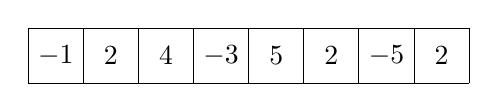
\begin{tikzpicture}[scale=0.7]
\draw (0,0) grid (8,1);

\node at (0.5,0.5) {$-1$};
\node at (1.5,0.5) {$2$};
\node at (2.5,0.5) {$4$};
\node at (3.5,0.5) {$-3$};
\node at (4.5,0.5) {$5$};
\node at (5.5,0.5) {$2$};
\node at (6.5,0.5) {$-5$};
\node at (7.5,0.5) {$2$};
\end{tikzpicture}
\end{center}
\begin{samepage}
この場合の最大の部分和は$10$です。
\begin{center}
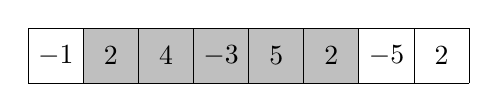
\begin{tikzpicture}[scale=0.7]
\fill[color=lightgray] (1,0) rectangle (6,1);
\draw (0,0) grid (8,1);

\node at (0.5,0.5) {$-1$};
\node at (1.5,0.5) {$2$};
\node at (2.5,0.5) {$4$};
\node at (3.5,0.5) {$-3$};
\node at (4.5,0.5) {$5$};
\node at (5.5,0.5) {$2$};
\node at (6.5,0.5) {$-5$};
\node at (7.5,0.5) {$2$};
\end{tikzpicture}
\end{center}
\end{samepage}

なお、空の配列も部分和と捉えるので$0$が考えられる最小の値となります。

\subsubsection{Algorithm 1}

この問題を解決する簡単な方法は、
可能性のあるすべての部分配列を調べ、
それぞれの部分配列の値の合計を計算し、
最大合計を計算することです。
次のコー ドはこのアルゴリズムを実装したものです。

\begin{lstlisting}
int best = 0;
for (int a = 0; a < n; a++) {
    for (int b = a; b < n; b++) {
        int sum = 0;
        for (int k = a; k <= b; k++) {
            sum += array[k];
        }
        best = max(best,sum);
    }
}
cout << best << "\n";
\end{lstlisting}

\texttt{a} と \texttt{b} で部分配列の両端を持ち、
その間の和を\texttt{sum}で計算します。
\texttt{best}はこの最大値を持つものです。

これは、ネストから推測できる通り、$O(n^3)$の計算量となります。

\subsubsection{Algorithm 2}

簡単に先ほどのコードからループを1つ撮ることができます。
右端を動かす時に和も計算して終えばいいのです。

\begin{lstlisting}
int best = 0;
for (int a = 0; a < n; a++) {
    int sum = 0;
    for (int b = a; b < n; b++) {
        sum += array[b];
        best = max(best,sum);
    }
}
cout << best << "\n";
\end{lstlisting}
こうすると、$O(n^2)$になりました。

\subsubsection{Algorithm 3}

驚くべきことに、この問題は $O(n)$ 時間で解くことができます
\footnote{In \cite{ben86}, this linear-time algorithm
is attributed to J. B. Kadane, and the algorithm is sometimes
called \index{Kadane's algorithm} \key{Kadane's algorithm}.}。
配列の各位置について,その位置で終了する部分配列の最大和を計算します。
この後,問題の答えは、それらの最大値となります。
位置$k$で終わる最大和の部分配列を求める補題を考えましょう。2つの可能性があります。

\begin{enumerate}
\item $k$のみが含まれる
\item $k-1$で終わる部分配列に加えて$k$が含まれる
\end{enumerate}

後者の場合、
総和が最大となる部分配列を求めたいので、
位置$k - 1$で終了する部分配列はそれまでの総和が最大となるはずです。
したがって、左から右へ各終了位置の最大の部分配列和を計算すれば、
この問題を効率的に解くことができるはずです。

実装を示します。
\begin{lstlisting}
int best = 0, sum = 0;
for (int k = 0; k < n; k++) {
    sum = max(array[k],sum+array[k]);
    best = max(best,sum);
}
cout << best << "\n";
\end{lstlisting}

ループが1つしかなく、$O(n)$で動作します。
この問題はどんな数字があるかを一度は確認しないといけないので、
考えうる最良の計算量と言えます。

\subsubsection{効率性の比較 - Efficiency comparison}

アルゴリズムが実際にどの程度効率的であるかを研究するのは興味深いポイントです。
次の表は、最新のコンピュータで、$n$の値を変えて上記のアルゴリズムを実行した場合の
実行時間です。

各テストでは、入力はランダムに生成し、入力の読み取り時間は測定していません。

\begin{center}
\begin{tabular}{rrrr}
array size $n$ & Algorithm 1 & Algorithm 2 & Algorithm 3 \\
\hline
$10^2$ & $0.0$ s & $0.0$ s & $0.0$ s \\
$10^3$ & $0.1$ s & $0.0$ s & $0.0$ s \\
$10^4$ & > $10.0$ s & $0.1$ s & $0.0$ s \\
$10^5$ & > $10.0$ s & $5.3$ s & $0.0$ s \\
$10^6$ & > $10.0$ s & > $10.0$ s & $0.0$ s \\
$10^7$ & > $10.0$ s & > $10.0$ s & $0.0$ s \\
\end{tabular}
\end{center}

この比較から、入力サイズが小さいときにはどのアルゴリズムも効率的だが、
入力サイズが大きくなると、アルゴリズムの実行時間に顕著な差が生じることがわかります。
アルゴリズム1は$n=10^4$のときに遅くなり、
アルゴリズム2は$n=10^5$のときに遅くなりました。
アルゴリズム3だけが、最大の入力でも瞬時に処理することができました。
